\chapter{Results and Evaluation}
\label{chap:res}
 \section {Testing Approach} 
For testing purposes  a corpus of  Verbmobil data (dialogues about meeting
appointments)  is available.  Each record contains audio file, used by the recognizer as input in
one of the configurations,  and \textit {gold standard}
with the true words from the audio, including true alignments.  Depending on the program configuration 
 the following types of outputs were available for evaluation:
\begin {enumerate}
  \item Google incremental output (1).
  \item Sphinx incremental output: Sphinx in recognition mode, using verbmobil
  or simplified language language model (2).
  \item Google+Sphinx: Sphinx in forced alignment mode after Google
  incrementally, alignment of the incremental results as described in the
  chapter \ref {chap:implem} (3).
  \item Google+Sphinx: Sphinx in forced alignment and recognition mode,
  combined alignment and phone loop grammar (4).
  \item Google+Sphinx: Sphinx in forced alignment and recognition mode,combined
  alignment grammar (5). 
\end{enumerate}
Alignment quality and timeliness were evaluated with the help of InTELiDA
(Incremental Timing Evaluation of Linguistic Data), providing \textit {Perl}
modules and a graphical user interface for incremental data analysis \parencite {baumann2013:phd}. For
alignment quality analyses a \textit {Perl} program, that computes the \textit {mean,
standard deviation and RMSE} as described in the chapter
\ref{chap:terms} was used. Timeliness metrics FO and FD were
evaluated, using graphical application of InTELiDA - \textit {interactivetool.pl}. 

\section {Test Results} 
\subsection {Alignment quality}
\begin {table}
\begin{center}
\caption {Alignments quality of the recognizer for matches and substitutions in
different configurations.}
    \begin{tabular}{l  c  c  c }
   \toprule
    Recognizer & mean & stddev & RMSE \\ \toprule
    Google (1)  & 1398 ms &  775 ms & 1672 ms \\ 
    Sphinx (2)  & 142 ms & 167 ms & 238 ms \\ 
    Google+Sphinx (3)  &  348  ms & 308 ms &  387 ms \\ 
    %Google+Sphinx (4)  & ms & ms & ms \\ 
    %Google+Sphinx (5)  & ms & ms & ms \\ 
    \bottomrule  
    \end{tabular}
    \label{tab:alnonincremm} 
\end{center}
\end {table}
\begin {table}
\begin{center}
\caption {Alignments quality of the recognizer only for matches 
in different configurations.}
    \begin{tabular}{l  c  c  c }
   \toprule
    Recognizer & mean & stddev & RMSE \\ \toprule
    Google (1)  & 1471 ms & 680 ms & 1735 ms \\ 
    Sphinx (2)  & 481 ms & 269 ms & 334 ms \\ 
    Google+Sphinx (3)  & 288 ms &  212 ms &  401 ms \\ 
    %Google+Sphinx (4)  & ms & ms & ms \\ 
    %Google+Sphinx (5)  & ms & ms & ms \\ \bottomrule  
    \end{tabular}
    \label{tab:alnonincremms}
\end{center} 
\end {table}
Results of the alignment quality analyses are shown in the tables above.
For analyses of the timing quality only Google+Sphinx in the forced alignment mode
was used. The first table \ref{tab:alnonincremm}   shows results for
matches and substitutions, whereas the table \ref{tab:alnonincremms}
shows results only for matches. Evaluation results for single files could be
found in the appendix \ref{chap:appC}. 

The quality of alignment, using Google+Sphinx has at least 400 \% increased,
whereas the the errors for \textit {mean, standard deviation and RMSE} are within the range of
400 ms. The results of Google+Sphinx are comparable with the results of Sphinx.
The alignment quality of Sphinx+ Google for matches is even better for the
analysed files than that of Sphinx. The difference is explained by the different
number of matches as well as matches and substitutions for Sphinx and for
Google+Sphinx.
% alone. The small difference between Sphinx+Google and Google is explained by the
% fact that the length of audio input, passed to Sphinx together with Google
% hypotheses is not always precisely computed. For future there should be
% considered a more sophisticated algorithm to compute the offset of Google. 

For incremental alignment quality analyses (compare chapter \ref{chap:terms})
only the first incremental result of the final output was considered. The results for Sphinx,
Google and Google+Sphinx in the alignment mode are presented in the tables
\ref{tab:alincrm} and \ref{tab:alincrms}. Results show that incremental
 alignment errors differs from errors with non-incremental approach in less than 5 \%. This fact supports the
argument that the incremental timing of Sphinx and Google+Sphinx
recognizers are as good as non-incremental timing of  Sphinx and Google+Sphinx
recognizers.
\begin {table}
\begin{center}
\caption {Incremental alignment quality of the recognizer for matches and 
substitutions in different configurations.}
    \begin{tabular}{ l  c  c  c }
    \toprule
    Recognizer & mean  & stddev & RMSE\\ \toprule
    Google (1)  & 823 ms & 540 ms & 1105 ms\\ 
    Sphinx (2)  &  145 ms & 215 ms & 234 ms \\ 
    Google+Sphinx (3) & 157 ms & 324 ms & 351 ms \\ 
    %Google+Sphinx (4)  & ms & ms & ms \\ 
    %Google+Sphinx (5)  & ms & ms & ms \\ 
    \bottomrule  
    \end{tabular}
    \label{tab:alincrm} 
\end{center}
\end {table}

\begin {table}
\begin{center}
\caption {Incremental alignment quality of the recognizer only for matches in
different configurations.}
    \begin{tabular}{ l  c  c  c }
    \toprule
    Recognizer & mean  & stddev & RMSE\\ \toprule
    Google (1)   & 808 ms & 456 ms & 1021 ms \\ 
    Sphinx (2)  &  474 ms & 211 ms & 320 ms \\ 
    Google+Sphinx (3)  & 199 ms & 189 ms & 311 ms \\ 
    %Google+Sphinx (4)  & ms & ms & ms \\ 
    %Google+Sphinx (5)  & ms & ms & ms \\ 
    \bottomrule  
    \end{tabular}
    \label{tab:alincrms} 
\end{center}

\end {table}
\subsection {Timeliness quality}
An example of the timeliness visualisation in InTEliDa is presented in the
figure \ref{fig:vis} . The figure shows the FO values for Sphinx output. 
\begin{figure}[htbp]
  \centering
    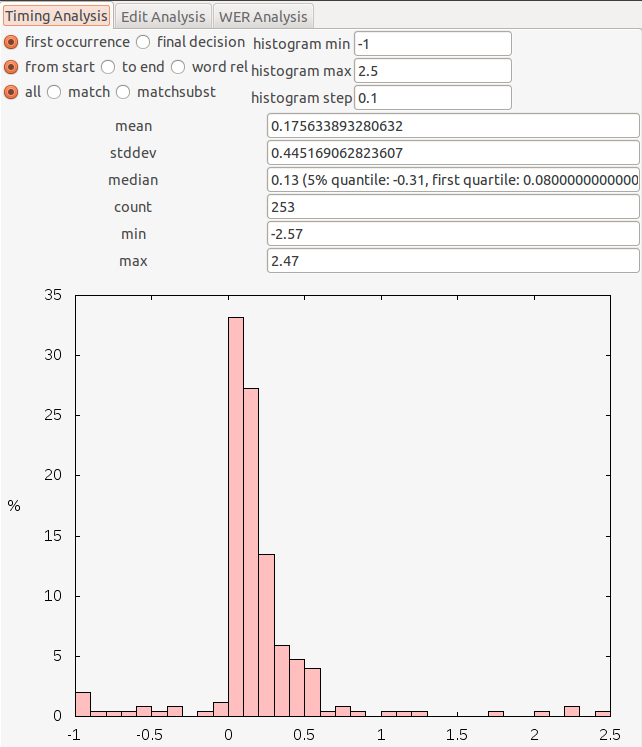
\includegraphics[width=1.0\textwidth]{images/sphinxFO.png}
 \caption{ FO analyses window in InTELiDa}
  \label{fig:vis}
\end {figure}
Results of the timeliness quality analyses are shown in the
tables below. The first table \ref {tab:FO} shows results for FO, whereas the
table  \label{tab:FD} shows results for FD.  The tables contain the results for
Google, Sphinx, and Google+Sphinx in alignment mode. 

As expected Sphinx demonstrates the best timeliness results, being at least 10
times faster in the recognition for the selected files. Google+Sphinx in the alignment
mode is slower as Google alone, as it waits for the first Google hypotheses to
start with the recognition. 

The results for Google+Sphinx in alignment +recognition mode were not
analysed. In case of JSGF Grammar the restriction was that phones could not be
directly compared to the \textit {gold standard} words.  For evaluation it is first
necessary, to convert the words of the first part of the
output and the words from \textit {gold standard} to phonemes.  Additionally,
timing should be calculated for every phoneme in the first part of the output. 
In this case FO and FD should be analysed on the level of phonemes.
Alternatively, there is a possibility to reconstruct the words from phonemes. 
 \begin {table}
\begin{center}
\caption {Timeliness quality of the recognizer in different configurations. FO
results.}
    \begin{tabular}{ l  c  c  c }
    \toprule
    Recognizer & mean & stddev & median \\ \toprule
    Google (1)  & 3202 ms & 3744 ms &  1466 ms\\
    Sphinx (2)  &175 ms & 445 ms & 130 ms \\
    Google+Sphinx (3)  & 2742 ms +offset  & 3787 ms + offset & 1000 ms + offset 
    \\
    %Google+Sphinx (4)  & ms & & \\ 
    Google+Sphinx (5)  & ms & &  \\ \bottomrule  
    \end{tabular}
    \label{tab:FO}
\end{center} 
\end {table}

Google+Sphinx in alignment and recognition, using a dynamic flat linguist, have
also shown a problem of incorrect timing computation for configurations with
dynamic flat linguist within InproTK. As a results the timing labels of the
results are not sequentially ordered in the first part of the graph and could
not be analysed by InTELiDa. For future development it is obligatory first to
improve recognition in Sphinx with dynamic flat linguist.  However, in spite of
non-sequentially ordered timing labels, the results show that Google+Sphinx
combination is able to improve Google timeliness by producing intermediate
results, while waiting for Google result, when the length of audio allows this. 
\begin {table}
\begin{center}
\caption {Timeliness quality of the recognizer in different configurations. FD
results.}
    \begin{tabular}{ l  c  c  c }
    %\hline
    \toprule
    Recognizer & mean & stddev & median \\ \toprule
    Google (1)  & 3702 ms & 4263 ms & 1705 ms  \\ 
    Sphinx (2)  & 213 ms & 445 ms & 150 ms \\ 
    Google+Sphinx (3)  & 2857 ms + offset & 3788 ms + 
    offset   & 1259 ms + offset \\
    %Google+Sphinx (4)  & ms  & & \\ 
    Google+Sphinx (5)  & ms  & &\\ \bottomrule   
    \end{tabular}
    \label{tab:FD} 
\end{center}
\end {table}

